% This is a sample LaTeX input file.  (Version of 12 August 2004.)
%
% A '%' character causes TeX to ignore all remaining text on the line,
% and is used for comments like this one.

\documentclass{article}      % Specifies the document class

\def\Course{Statistical Methods for Machine Learning}
\def\Exam{Assignment 1}
\def\Studentname{
Tudor Dragan (xlq880)\\
Nicolae Mariuta (rqt629)\\
Gabriel Carp (slp670)
}
\def\Sub_date{\today}
                             % The preamble begins here.
%\title{\bf Principles of Computer Systems Design\\ {\Large Exam}}  % Declares the document's title.
%\author{Tudor Dragan\\}

\title{\textbf{\Course}\\\textbf{\Exam}}
\author{\Studentname}
\date{\Sub_date}      % Deleting this command produces today's date.

\usepackage{verbatimbox}
\usepackage{listings}
\usepackage{color}
\usepackage[]{amsmath}
\usepackage[english]{babel}
\usepackage[utf8]{inputenc}
\usepackage{graphicx}
\usepackage{moreverb}
\usepackage{hyperref}
\usepackage[T1]{fontenc} % font
\usepackage{program}
\usepackage[top=1.5in, bottom=1.5in, left=1.4in, right=1.4in]{geometry}
\usepackage[super]{nth}
\usepackage{fancyhdr}
\usepackage{lastpage}
\usepackage{float}
\usepackage[section]{placeins}
\usepackage[linesnumbered]{algorithm2e}
\usepackage[table,xcdraw]{xcolor}
\definecolor{dkgreen}{rgb}{0,0.6,0}
\definecolor{gray}{rgb}{0.5,0.5,0.5}
\definecolor{mauve}{rgb}{0.58,0,0.82}
\usepackage[table,xcdraw]{xcolor}
\lhead{\textbf{\Course}}
\rhead{\Exam~(Submission: \Sub_date)}

\cfoot{}
\lfoot{\Studentname}
\rfoot{\thepage\ of \pageref{LastPage}}
%\pagestyle{fancy}
\renewcommand{\footrulewidth}{0.4pt}

\lstset{frame=tb,
      language=Java,
      aboveskip=3mm,
      belowskip=3mm,
      showstringspaces=false,
      columns=flexible,
      basicstyle={\small\ttfamily},
      numbers=none,
      numberstyle=\tiny\color{gray},
      keywordstyle=\color{blue},
      commentstyle=\color{dkgreen},
      stringstyle=\color{mauve},
      breakatwhitespace=true
      tabsize=3
}
\newcommand{\ip}[2]{(#1, #2)}
                             % Defines \ip{arg1}{arg2} to mean
                             % (arg1, arg2).

%\newcommand{\ip}[2]{\langle #1 | #2\rangle}
                             % This is an alternative definition of
                             % \ip that is commented out.

\begin{document}             % End of preamble and beginning of text.

\maketitle                   % Produces the title.

\section*{I.2 Probability and Parameter Estimation}
\subsection*{I.2.1 Univariate Gaussian distributions}

\begin{figure}[ht]
\centering
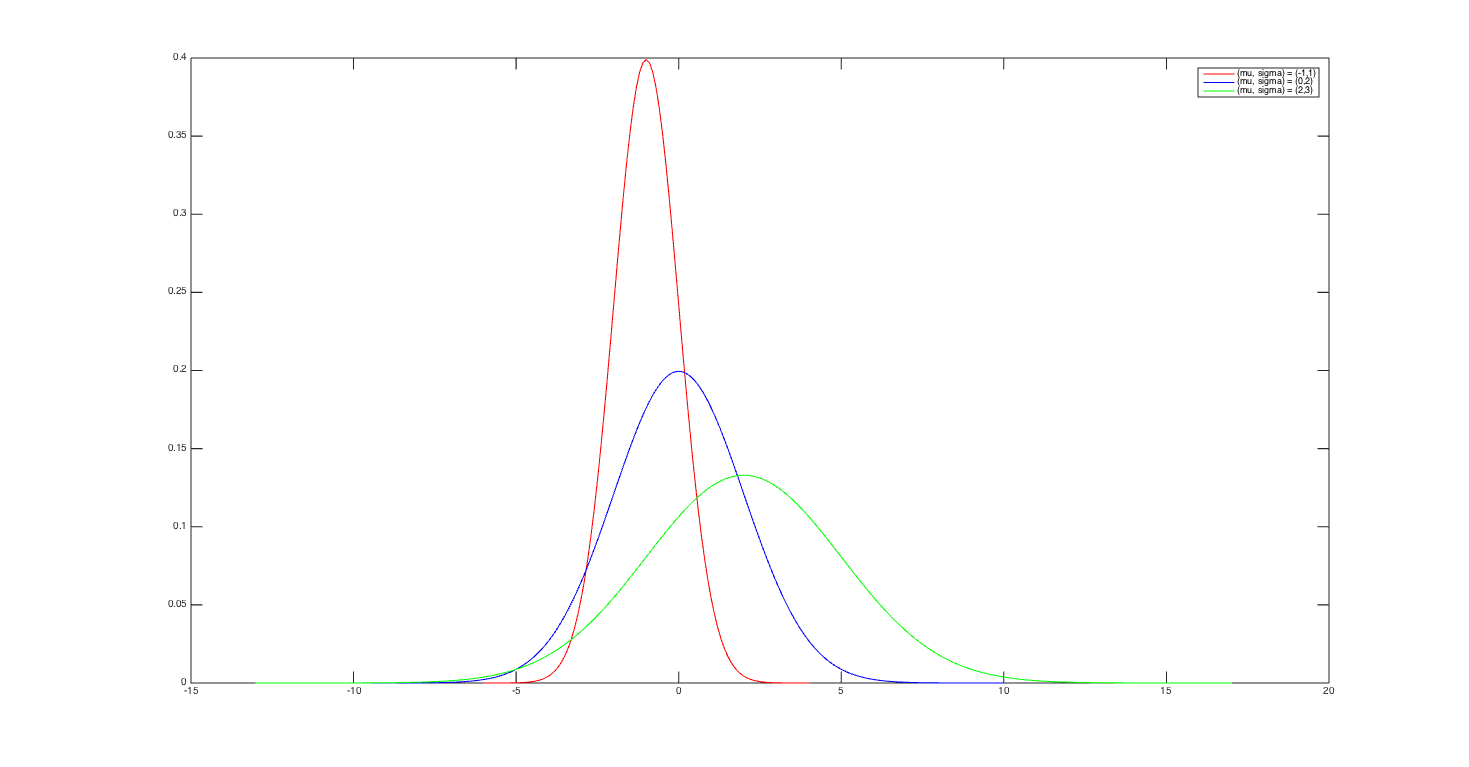
\includegraphics[scale=.3]{img/i21}
\caption{Gaussian distribution for  \label{overflow}}
\[(\mu,\sigma) = (-1, 1), (0, 2), and (2, 3)   \]
\end{figure}

Ox in the gaussian1d function represents the input values and Oy is the output that is calculated by applying the univariate Gaussian Distribution function with means m and standard deviation d.\\

\subsection*{I.2.2 Sampling from a multivariate Gaussian distribution}

\begin{figure}[ht]
\centering
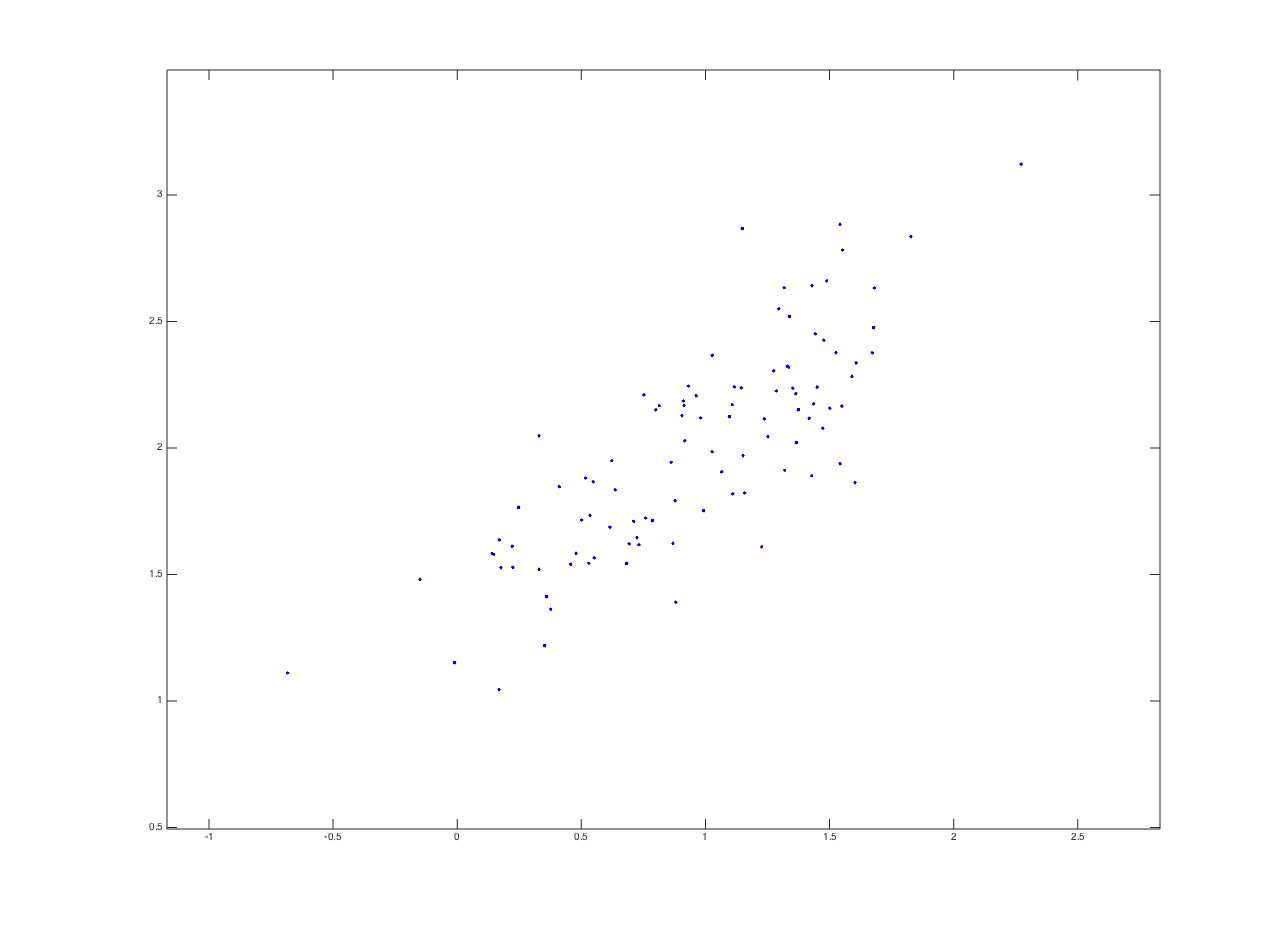
\includegraphics[scale=.3]{img/i22}

\caption{The plot for the input data set \label{overflow}}
\end{figure}

\subsection*{I.2.3 Means}

\begin{figure}[ht]
\centering
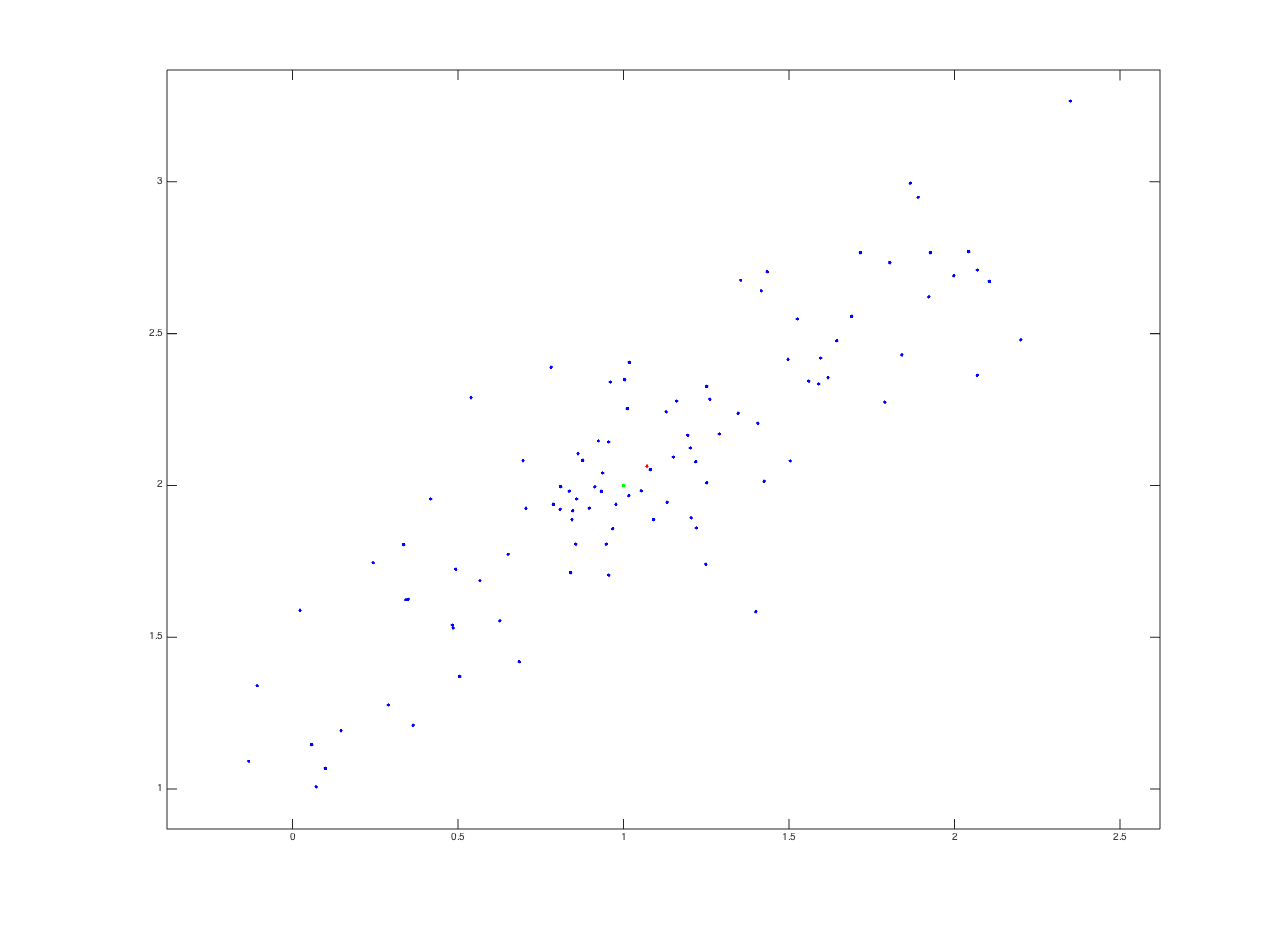
\includegraphics[scale=.3]{img/i23}
\caption{The two means: sample mean (green) and quantitive mean (red) \label{overflow}}
\end{figure}

In Figure 3 we have represented the two means: mu which is the given mean ([1, 2]) and m is the quantitive mean that has been calculated by calculating the average of all the points in the data set. Because we generate the data set randomly, the points are chosen independently from each other. Because of this we have this deviation between the sample mean and the quantitive one. If we would have had a sample that was based on a periodical function, then the mean would have been identical because it would comply to the same rule. Furthermore, the smaller the number of our data set the bigger the deviation gets because we would have larger granularity between the set of values. So if we would have an infinite number of data points we would have "almost" the same mean.\\

\subsection*{I.2.4 Covariance: The geometry of multivariate Gaussian distributions}
The covariance is the property of a function of retaining its form when the variables are linearly transformed. Therefore if we rotate the data set by 30, 60 or 90 degrees we should get the elliptic shape as the standard data set. In our case, the covariance is a matrix of size (2,2) represented in the following:\\

\[
Cov\ \Sigma_{ML}
=
\begin{bmatrix}
    0.4012       & 0.2798  \\
   0.2798       & 0.2614 \\
\end{bmatrix}
\]\\

The major axes of the ellipse are defined by the eigenvectors of the covariance matrix, with corresponding eigenvalues. The main direction of the data sampled from the Gaussian distribution points along the x axis for \[\alpha = -2.478 \] as seen in Figure 5.\\

\begin{figure}[h]
\centering
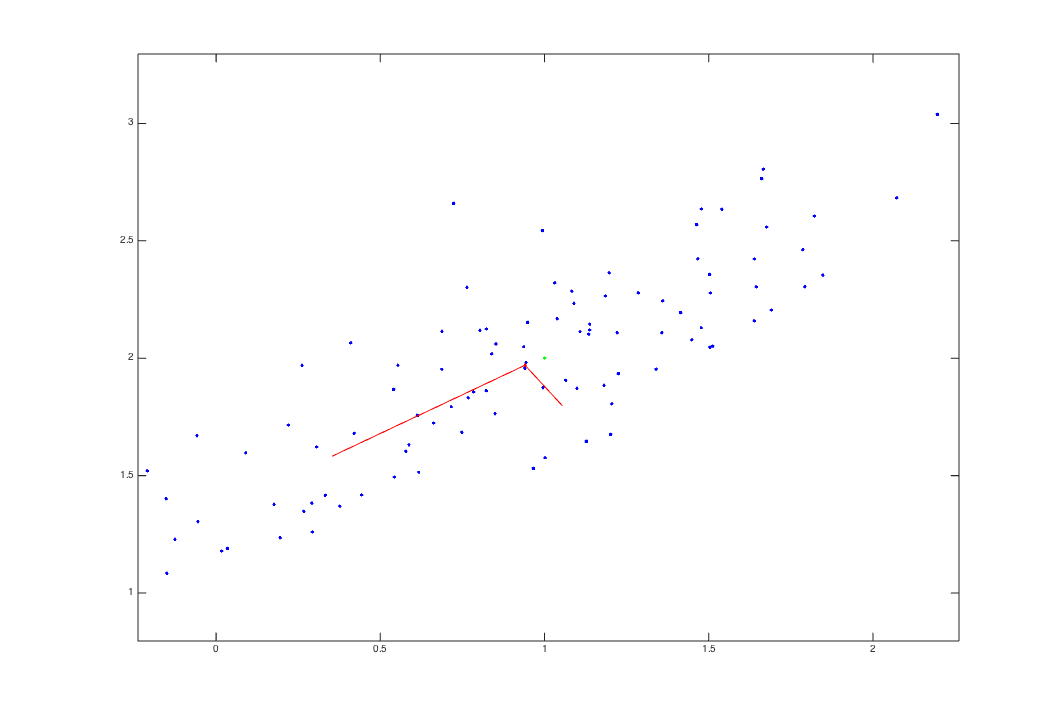
\includegraphics[scale=.3]{img/i24}
\caption{Covariance and eigenvectors \label{overflow}}
\end{figure}

\begin{figure}[h]
\centering
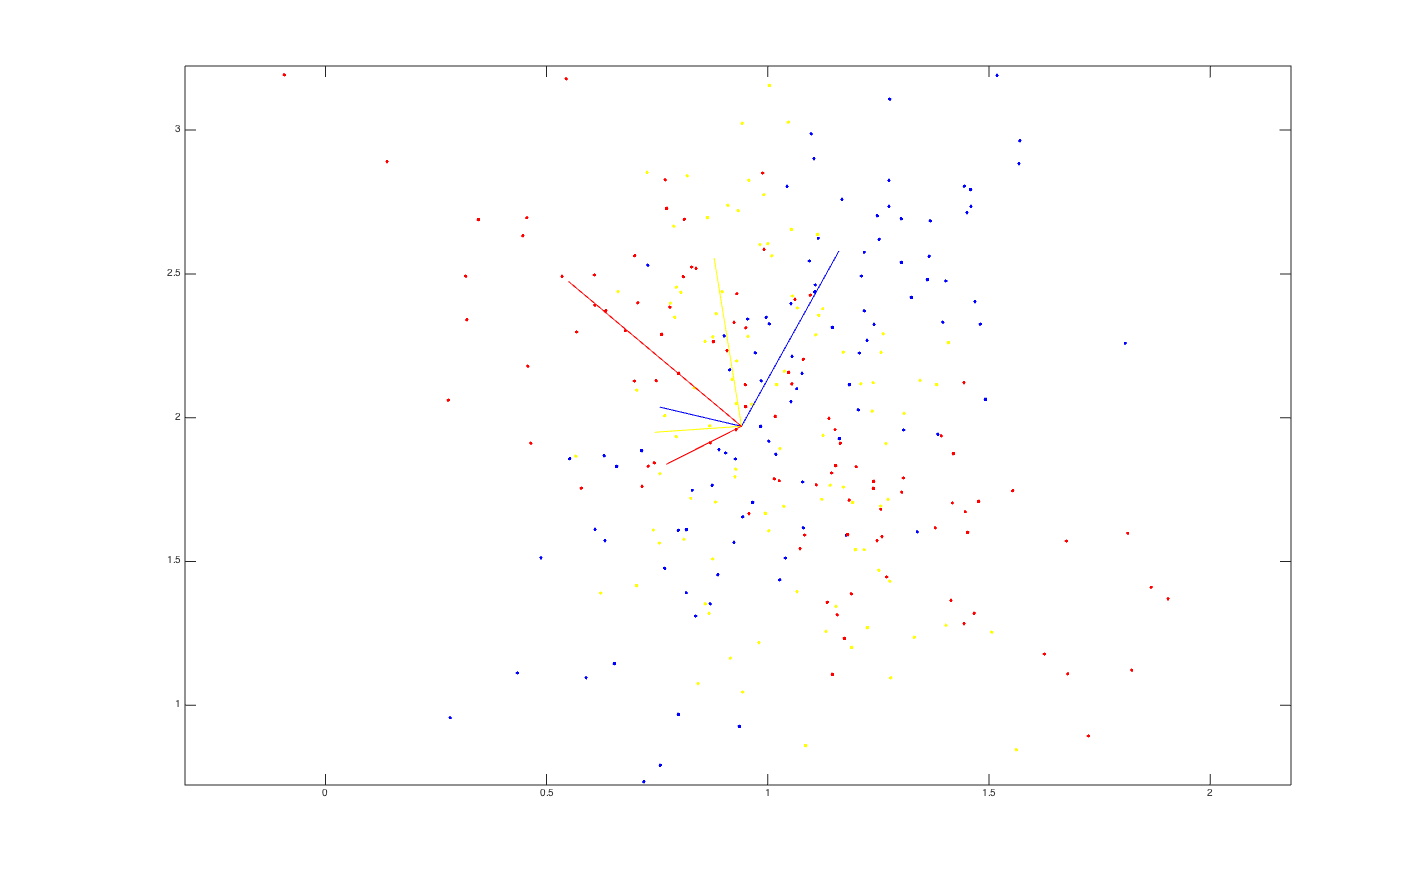
\includegraphics[scale=.2]{img/i24b}
\caption{Combined plot of rotated datasets \label{overflow}}
\end{figure}

\section*{I.3 Classification}
\subsection*{I.3.1 Nearest neighbor}
 
The kNN function is applied for K = \{1, 3, 5\}. The kNN function starts out by calculating the distances for each point in the test data relative to the train data points. After that, we sort the rows by distance and create a counting vector that holds the K number of points that are closest to the current analyzed point. We check then the highest count in the vector and calculate the accuracy (1 - empirical risk) by checking the values from the train and test data sets.\\

\begin{table}[h]
\begin{center}
\begin{tabular}{|
>{\columncolor[HTML]{000000}}c |c|c|c|}
\hline
{\color[HTML]{FFFFFF} \textbf{K}}    & 1      & 3      & 5 \\ \hline
{\color[HTML]{FFFFFF} \textbf{Training Data}} & 0.770 & 0.7700 &  0.7400 \\ \hline
{\color[HTML]{FFFFFF} \textbf{Test Data}} & 0.8158 & 0.8158 &  0.6842 \\ \hline
\end{tabular}
\caption{K-NN accuracy values}
\label{K-NN accuracy values}
\end{center}
\end{table}

\subsection*{I.3.2 Hyper-parameter selection using cross-validation}

For the cross validation we split the train data matrix into 5 parts. We took a k from 1 to 25 with step set to 2 and applied the cross validation algorithm like so:

\begin{itemize}
\item
We exclude one part at a time from the train matrix and apply the kNN function on the part left out as the test data.
\item 
We calculate the average k and add it to the kRiskMatrix.
\item
The last step searches for the minimum risk for a given k ($k_{best}$).
\item
In our case, the best value of k should be 3.
\end{itemize}

The entire kRiskMatrix can be seen in Table 2.\\

% Please add the following required packages to your document preamble:
% \usepackage[table,xcdraw]{xcolor}
% If you use beamer only pass "xcolor=table" option, i.e. \documentclass[xcolor=table]{beamer}
\begin{table}[h]
\begin{center}
\begin{tabular}{|
>{\columncolor[HTML]{333333}}c |c|c|c|c|c|c|c|c|c|c|c|c|l|}
\hline
{\color[HTML]{FFFFFF} \textbf{K}}    & 1    & 3    & 5    & 7    & 9    & 11   & 13   & 15   & 17   & 19   & 21   & 23   & 25   \\ \hline
{\color[HTML]{FFFFFF} \textbf{Risk}} & 0.22 & 0.20 & 0.25 & 0.22 & 0.22 & 0.22 & 0.22 & 0.21 & 0.21 & 0.22 & 0.21 & 0.22 & 0.21 \\ \hline
\end{tabular}
\caption{Number of neighbors as suggested by hyperparameter selection}
\label{Number of neighbors as suggested by hyperparameter selection}
\end{center}
\end{table}

\subsection*{I.3.3 Data normalization}

After the normalization the two parameters reside in almost the same interval and that's why both parameters have the same weight in the classification algorithm. Before normalization, one of the parameters had values between 4 and 7 and the second one had values between 0.20 and 0.40. Because of this the second parameter had a smaller effect in the classification's performance. We applied the normalization by calculating the mean for the train data set and the standard deviation for each parameter by applying the function in the lecture slides. \\

The means and variances for the untransformed data are shown here:\\

\[
mean_{train} 
=
\begin{bmatrix}
    5.766       & 0.301  \\
\end{bmatrix}
\]
\[
stdDev_{train}
=
\begin{bmatrix}
    0.830       & 0.041  \\
\end{bmatrix}
\]
\[
mean_{test} 
=
\begin{bmatrix}
    5.928       & 0.319  \\
\end{bmatrix}
\]
\[
stdDev_{test}
=
\begin{bmatrix}
    0.859       & 0.046  \\
\end{bmatrix}
\]\\

The means and variances for the normalized data are shown here:\\

\[
mean_{train} 
=
\begin{bmatrix}
    ~0      & ~0  \\
\end{bmatrix}
\]
\[
stdDev_{train}
=
\begin{bmatrix}
    1       & 1  \\
\end{bmatrix}
\]
\[
mean_{test} 
=
\begin{bmatrix}
    ~0       & ~0  \\
\end{bmatrix}
\]
\[
stdDev_{test}
=
\begin{bmatrix}
    1.036       & 1.119  \\
\end{bmatrix}
\]\\
 
 
 The error for the training and the test data is as follows:\\
 
 \begin{table}[h]
\begin{center}
\begin{tabular}{|
>{\columncolor[HTML]{000000}}c |c|c|c|}
\hline
{\color[HTML]{FFFFFF} \textbf{$K_{Best}$}}    & 3  \\ \hline
{\color[HTML]{FFFFFF} \textbf{Training Data}} & 0.070  \\ \hline
{\color[HTML]{FFFFFF} \textbf{Test Data}} & 0.1842  \\ \hline
\end{tabular}
\caption{Error for $k_{Best} = 3$}
\label{Error for $k_{Best} = 3$}
\end{center}
\end{table}

The $f_{norm}$ function is represented in our code as $f_{norm} = (X -mean(X)) / std(X)$. After obtaining this function we also normalized the test set and applied the methods from the previous exercise for finding $k_{best}$. After that we calculated the empirical error. Our results show that $k = 1$ is the argmin for the test set and the standard deviation is a little higher (0.23). We also have noticed that for $k = 3$ the empirical error is lower. That is probably because our data set is not large enough and the result should be better if we would have a much larger data test set.\\

\end{document}               % End of document.